\documentclass{estilo}
\usepackage[spanish]{babel}
\usepackage{graphicx}
\usepackage{float}
\usepackage{amsmath}        % para los vectores columnas
\usepackage{amsfonts}       % para las negrita de pizarra
\usepackage{amssymb}        % para simbolos matematicos
\usepackage{hyperref}       % para utilizar referencias
\usepackage{multirow}       % para las tablas
\usepackage{dsfont}
\usepackage{listings}
\usepackage{xcolor}
\definecolor{codegreen}{rgb}{0,0.6,0}
\definecolor{codegray}{rgb}{0.5,0.5,0.5}
\definecolor{codepurple}{rgb}{0.58,0,0.82}
\definecolor{backcolour}{rgb}{0.95,0.95,0.92}
\lstdefinestyle{mystyle}{
    backgroundcolor=\color{backcolour},   
    commentstyle=\color{codegreen},
    keywordstyle=\color{magenta},
    numberstyle=\tiny\color{codegray},
    stringstyle=\color{codepurple},
    basicstyle=\ttfamily\footnotesize,
    breakatwhitespace=false,         
    breaklines=true,                 
    captionpos=b,                    
    keepspaces=true,                 
    numbers=left,                    
    numbersep=5pt,                  
    showspaces=false,                
    showstringspaces=false,
    showtabs=false,                  
    tabsize=2
}
\lstset{style=mystyle}

\usepackage{enumitem,multicol,setspace}
\newcounter{subenum}[enumi] % para las multicolumnas
\renewcommand{\thesubenum}{\arabic{subenum}}
\usepackage[nomessages]{fp}
\FPeval\thecolwidth{round(1/4:4)}% Specify number of columns -> column width
\newcommand{\newitem}[1]{%
  \refstepcounter{subenum}%
  \parbox{\dimexpr\thecolwidth\linewidth-.5\columnsep}{%
    \makebox[\labelwidth][r]{(\thesubenum)\hspace*{\labelsep}}%
    #1}\hfill%
}

\usepackage{scalerel,stackengine} % para el sombrero
\stackMath
\newcommand\rhat[1]{%
\savestack{\tmpbox}{\stretchto{%
  \scaleto{%
    \scalerel*[\widthof{\ensuremath{#1}}]{\kern-.6pt\bigwedge\kern-.6pt}%
    {\rule[-\textheight/2]{1ex}{\textheight}}%WIDTH-LIMITED BIG WEDGE
  }{\textheight}% 
}{0.5ex}}%
\stackon[1pt]{#1}{\tmpbox}%
}
\parskip 1ex

\usepackage{mathtools}      % floor y ceil
\DeclarePairedDelimiter\ceil{\lceil}{\rceil}
\DeclarePairedDelimiter\floor{\lfloor}{\rfloor} 

\usepackage[style=authoryear-comp]{biblatex}


\begin{document}
\maketitle

\justifying{}

\newpage
\section{Introduccion}

El problema que se nos plantea es que el tiempo total para poder analizar todos los siguientes \textbf{\textit {n}} rivales del \textbf{CAMPEÓN DEL MUNDO} sea el más óptimo. A su vez, se solicita que sea hallado con un algoritmo Greedy. Para tener en mente, los algoritmos Greedy siguen una regla sencilla que les permiten obtener un \textit{óptimo local} según el estado actual del programa, y poder llegar a un \textit{óptimo general} juntando los locales. Pero como todo, pueden tener sus ventajas y desventajas, como por ejemplo que no siempre dan el resultado óptimo, o que demostrar que el resultado es óptimo es difícil. Por otro lado, son intuitivos de pensar y fácil de entender, y suelen ser rápidos. Lo que en reglas generales suele indicar que el algoritmo es Greedy es el uso de colas de prioridad como el \textit{heap} u ordenamientos (recalcar que un algoritmo puede hacer uso de heaps u ordenamientos y no ser Greedy).

Dicho esto, empezamos a plantear posibles soluciones para el problema. Lo primero que se nos vino a la idea es hacer uso de algún tipo de ordenamiento, ya sea ordenando por los tiempos de Scaloni o los ayudantes, en relación a cuánto tardaría cada uno. Lo que nos ayudó a volcarnos por el lado de ordenar por los tiempos de los ayudantes fue el siguiente:
\begin{itemize}
	\item El tiempo total que tarda Scaloni siempre va a ser el mismo, no importa cómo ordenemos los videos a ver. Bien como se dice, \textit{"El orden de los factores no altera el producto"}.
	\item Por más que Scaloni termine de ver el último video del último rival, va a quedar que después un ayudante analice el video, por lo que es más importante el tiempo que va a tardar este último ayudante que el que va a tardar Scaloni.
\end{itemize}

Ahora bien, ya tenemos definido por donde queremos encarar el problema, pero todavía falta definir en qué orden queremos que los videos se visualicen dependiendo de los ayudantes, si los más rápidos primero o viceversa. Acá entra en juego un factor muy importante a tener en cuenta: \textbf{los ayudantes analizan los videos inmediatamente termina Scaloni de ver el video, y el análisis de cada ayudante es independiente a los otros}. Esto quiere decir que si Scaloni terminó un video, inmediatamente uno de los ayudantes se pondrá a analizarlo. Y si Scaloni termina otro video, otro ayudante podrá empezar a analizar ese video, no importa si el anterior terminó de realizar su análisis o no. Esto nos ha llevado a tomar la decisión de ordenar por el tiempo de los ayudantes del que más tarde al que menos, por los siguientes puntos:
\begin{itemize}
	\item Los ayudantes pueden analizar un video independientemente de si el anterior haya terminado o no su análisis.
	\item Si para el último video queda el ayudante que mas tarda, el tiempo total no seria el optimo sino todo lo contrario, ya que se tardaría el tiempo total de Scaloni más lo que tarde este último.
	\item Por ese motivo, conviene que los ayudantes que más tarden estén al principio, ya que tienen tiempo hasta que Scaloni termine todos los videos para terminar. Y los ayudantes que menos tardan, estarán al final, de modo que si Scaloni termina, los que les falten sabemos que son los más rápidos y terminan lo antes posible.
\end{itemize}

\newpage
\justifying{
\section{Algoritmos}

A continuación se detallan los códigos y los pasos que se siguieron para llevar a cabo los algoritmos planteados utilizando distintas tecnicas de programacion.

\subsection{Backtracking}

A continuación se detallan el código y los pasos que se siguieron para llevar a cabo el algoritmo planteado utilizando \textbf{\textit{Backtracking}}.

\subsubsection{Obtener las posibles soluciones}

Una vez se obtuvieron todos los subconjuntos de jugadores para cada partido:

\lstinputlisting[language=Python]{code/backtracking.py}

siendo:
\begin{itemize}
    \item $A$: Lista compuesta de $m$ listas, las cuales representan un conjunto de jugadores para jugar un partido.
    \item \texttt{jugadores}: Lista con un subconjunto de jugadores que representan una posible solucion actual.
    \item \texttt{soluciones}: Lista con todos los subconjuntos de jugadores que son soluciones.
    \item \texttt{n}: Numero que indica sobre cual de las $m$ listas estamos trabajando.
    \item \texttt{utilizados}: Diccionario cuyo par \textit{clave-valor} es \textit{jugador-n} donde $n$ representa la enesima-lista en la que fue utilizado el jugador.\footnote{Siendo $n$ el menor valor encontrado hasta el momento}
    \item \texttt{minimo}: El minimo es un numero que representa la longitud del subconjunto mas pequeño que se encuentra en soluciones. (Se utiliza dentro de una lista dado que las listas actuan como punteros)
\end{itemize}

El algoritmo persigue la exploración de diversas soluciones mediante combinaciones, las cuales se ven restringidas mediante condiciones de poda. Este enfoque se implementa con el propósito de evitar la evaluación exhaustiva de todas las posibles combinaciones evitando que se convierta en un algoritmo de \textit{Fuerza Bruta}, optimizando así la eficiencia del proceso.

Estas condiciones de poda son:
\begin{itemize}
	\item En caso de que la longitud de la solución actual sea igual o mayor que la longitud de la solución óptima encontrada hasta el momento, se concluye que la solución actual no mejorará la situación. La igualdad se justifica porque, al estar en esta línea de código, implica que aún quedan listas por recorrer. En estas listas, podría agregarse un elemento más, lo cual invalidaría la condición de optimalidad. En el caso de no agregarlo, no se habría encontrado una solución mejor.
	\item En el caso de que un elemento de la solución actual pertenezca al subconjunto bajo análisis, se concluye que no es necesario explorar soluciones adicionales que involucren elementos de dicho subconjunto. dado que nuestro objetivo es usar la menor cantidad de elementos en la solucion final.
	\item Si un jugador ya fue utilizado en un nivel mas alto del arbol de posibilidades, entonces ya cubrio todas las combinaciones que vengan en niveles inferiores. En consecuencia, si se detecta la presencia de dicho jugador en un nivel menor al que se había identificado previamente, se interrumpe la exploración de nuevas combinaciones con este elemento, dado que su participación ya ha sido exhaustivamente considerada en niveles superiores.
\end{itemize}

En cuanto a la complejidad del algoritmo, este analiza exhaustivamente todas las combinaciones posibles. No obstante, interrumpe el procesamiento de aquellas combinaciones que no conducen a una solución óptima, lo que, en consonancia con la propia naturaleza del enfoque de backtracking, implica una complejidad de ${O}(2^n)$, dada su relación con la exploración de todas las combinaciones posibles. 

\subsubsection{Obtener la solucion optima de todas las ya encontradas}

Para obtener la solucion optima se implementó el siguiente algoritmo:

\lstinputlisting[language=Python]{code/optima.py}

El codigo lo unico que hace una vez imvocada a la funcion es buscar la minima solucion en base a la longitud.


\subsection{Programacion Lineal}





\subsection{Algoritmo Greedy}

Para poder ir al codigo, primero recordemos como funciona un algoritmo Greedy. Los algoritmos Greedy siguen una regla sencilla que les permiten obtener un \textit{óptimo local} según el estado actual del programa, y poder llegar a un \textit{óptimo general} combinando los locales. A su vez presentan desventajas, como por ejemplo que no siempre dan el resultado óptimo, o que demostrar que el resultado es óptimo es difícil. Por otro lado, son intuitivos de pensar y fácil de entender, y suelen ser eficientes.

Ahora bien, nuestra regla sencilla se baso en lo siguiente:
\begin{itemize}
    \item Para cada uno de los elementos, en nuestro caso jugadores, se iterara el resto de subconjuntos, que en este caso seran los pedidos de los demas medios.
    \item Se tomara el jugador que mas medios represente y pueda hacernos quedar bien con ellos. Estos medios ya se desestimaran porque ya habra un jugador que ellos desean ver.
    \item En caso de que la actual iteracion sea de un medio que ya esta considerado ya que uno de sus jugadores fue tomado en cuenta, se continuara sin analizarlo.
\end{itemize}

Esto hara lo mejor posible teniendo en cuenta la informacion actual del programa ya que siempre buscara el mejor jugador que pueda satisfacer la mayor cantidad de medios posibles.

El codigo es el siguiente:

\lstinputlisting[language=Python]{code/greedy.py}

El codigo funciona de la siguiente manera:
\begin{itemize}
    \item \texttt{b}: set de subconjuntos que recibimos. Cada subconjunto representaria los pedidos de los medios.
    \item \texttt{res}: set de resultado, aqui se aniadiran todos los jugadores que deben meterse si o si en el plantel si Scaloni no quiere problemas con ningun medio.
    \item \texttt{considered}: set de medios que se van considerando a medido que aniadimos jugadores a nuestro set de resultado.
    \item Para cada $subset$ se itera sus elementos, que aqui seran los pedidos de los medios y los jugadores que desean ver. Para cada jugador del medio que se esta iterando, se iteran los que quedan por ver, y nos guardaremos los medios que abarcara cada jugador para luego desestimarlos ya que estaran siendo considerados al elegir al jugador que mas abarque medios.
    \item cuando se termina de iterar dicho medio, se agrega todos los medios del jugador que mas abarca al set de medios considerados, asi ahora en adelante esos no se tienen en cuenta para calcular la eficiencia de un jugador al determinar que tanto nos aportara si lo metemos o no.
\end{itemize}

La complejidad de dicho algoritmo es $\mathcal{O}\left(n^2 \times m^2\right)$ siendo $n$ la cantidad de subsets (pedidos de los medios) y $m$ la cantidad de elementos (jugadores) ya que por cada subset se itera cada elemento, y por cada elemento se itera $n-1$ subsets y por cada uno de esos subsets todos sus elementos.
\section{Mediciones}

Se realizaron mediciones en base a crear pruebas de distintos tamaños y tomar su tiempo de ejecución individualmente, y en base a los datos recolectados hacer el gráfico. Los datos fueron desde 2000 hasta 20.000 elementos, los cuales las ganancias de cada entrenamiento fue generada aleatoriamente entre valores de 1 y 100, y para las energías fueron decayendo en porcentajes. Es decir, el 1\% del total fue 100, otro 99, otro 98... hasta llegar a 1. De esta manera, nos aseguramos de que cada día seguido entrenando cumple con la condición de que la energía de ese día es \textbf{menor o igual} al anterior.

\begin{figure}[H]
    \centering
    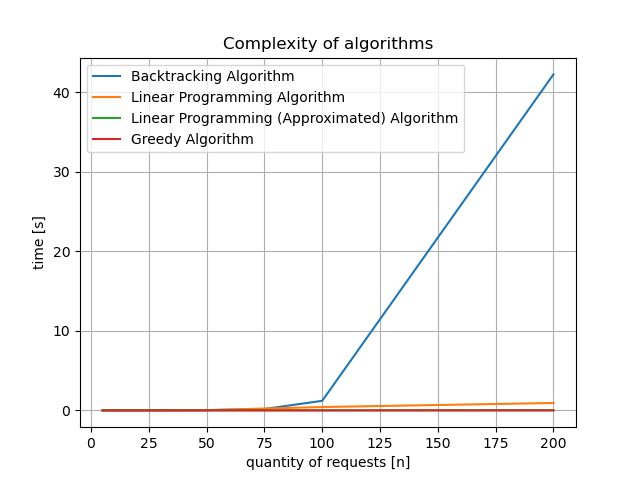
\includegraphics[width=0.9\textwidth]{img/graphic.png}
\end{figure}

Como se puede apreciar, el algoritmo planteado con \textit{Programación Dinámica} efectivamente cumple con la complejidad indicada anteriormente, ya que su diferencia con la complejidad de $\mathcal{O}(n \times n)$ es casi nula\footnote{Aclaración: para la complejidad indicada por la traza perteneciente a $\mathcal{O}(n \times n)$, se ha dado cierto valor al parámetro $a$ en la ecuación $y=ax^2$ ya que sino para 20.000 elementos el valor $y$ sería igual a 400.000.000, haciendo parecer que nuestro algoritmo es constante.}.

\section{Conclusiones}


En resumen, hemos logrado optimizar significativamente el tiempo requerido para analizar a todos los rivales mediante la implementación de un algoritmo Greedy. Este enfoque nos ha permitido descomponer el problema general en partes más manejables, lo que ha simplificado su resolución gradual y ha reducido considerablemente la complejidad computacional. Como resultado, hemos evitado la necesidad de analizar todos los posibles escenarios exhaustivamente.

Además, hemos respaldado con mediciones empíricas que confirman la eficiencia y la complejidad esperada. Estos resultados refuerzan la validez y la utilidad de nuestra estrategia para abordar problemas complejos de manera efectiva y eficiente.


Finalmente, valoramos la oportunidad de colaborar en esta tarea crucial y estamos determinados a contribuir al éxito continuo de la selección campeona del mundo.




}


\newpage
\end{document}